\section*{Seminár 11}
\subsection*{Téma}
Geometria III -- obsahy trojuholníkov a štvoruholníkov

\subsection*{Ciele}
Precvičenie úloh zaoberajúcich sa obsahmi trojuholníkov a štvoruholníkov,  rôznorodé určovanie obsahu, príp. pomeru obsahov trojuholníkov v~úlohách.

\subsection*{Úlohy a riešenia}
\begin{tcolorbox}[breakable,notitle,boxrule=0pt,colback=light-gray,colframe=light-gray]\ul{11.1} [57-S-2] V~danom rovnobežníku $ABCD$ je bod $E$ stred strany $BC$ a bod $F$ leží vnútri strany $AB$. Obsah trojuholníka $AFD$ je $15$\,cm$^2$ a obsah trojuholníka $FBE$ je $14$\,cm$^2$. Určte obsah štvoruholníka $FECD$.

\end{tcolorbox}

\rieh Označme $v$ vzdialenosť bodu $C$ od priamky $AB$, $a = |AB|$ a $x = |AF|$. Pre obsahy trojuholníkov $AFD$ a $FBE$ (obr. 1) platí $\frac{1}{2}x\cdot v~= 15$, $\frac{1}{2}(a - x) \cdot \frac{1}{2}v = 14$. Odtiaľ $xv = 30$, $av - xv = 56$. Sčítaním oboch rovností nájdeme obsah rovnobežníka $ABCD$: $S_{ABCD} = av = 86$\,cm$^2$. Obsah štvoruholníka $FECD$ je teda $S_{FECD} = S_{ABCD}- (S_{AFD} + S_ {FBE}) = 57$\,cm$^2.$
\begin{center}
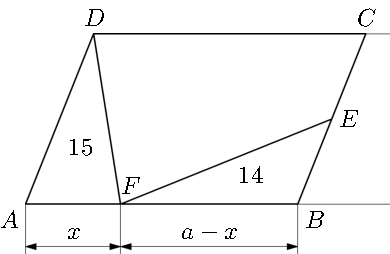
\includegraphics{obrazky/57S21} 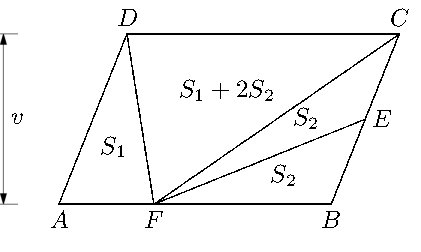
\includegraphics{obrazky/57S22}\\

Obr. 1  \ \ \ \ \ \hspace{130pt} Obr. 2
\end{center}
\textbf{Iné riešenie.} Trojuholníky $BEF$ a $ECF$ majú spoločnú výšku z~vrcholu $F$ a zhodné základne $BE$ a $EC$. Preto sú obsahy oboch trojuholníkov rovnaké. Z~obr. 2 vidíme, že obsah trojuholníka $CDF$ je polovicou obsahu rovnobežníka $ABCD$ (oba útvary majú spoločnú základňu $CD$ a rovnakú výšku). Druhú polovicu tvorí súčet obsahov trojuholníkov $AFD$ a $BCF$. Odtiaľ $S_{FECD} = S_{ECF} + S_{CDF} = S_{ECF} + (S_{AFD} + S_{BCF}) = S_{AFD} + 3 S_{FBE} = 57$\,cm$^2$.\\
\\
\textbf{Iné riešenie.} Do rovnobežníka dokreslíme úsečky $FG$ a $EH$ rovnobežné so stranami $BC$ a $AB$ tak, ako znázorňuje obr. 3.
\begin{center}
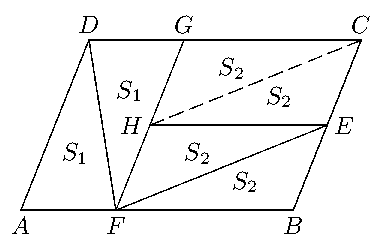
\includegraphics{obrazky/57S23}\\

Obr. 3
\end{center}
Rovnobežníky $AFGD$ a $FBEH$ sú svojimi uhlopriečkami $DF$ a $EF$ rozdelené na dvojice zhodných trojuholníkov. Takže $S_{GDF} = S_{AFD} = 15$\,cm$^2$ a $S_{HFE} = S_{BEF} = 14$\,cm$^2$. Zo zhodnosti rovnobežníkov $HECG$ a $FBEH$ navyše ľahko usúdime, že všetky štyri trojuholníky $FBE$, $EHF$, $HEC$ a $CGH$ sú zhodné, takže obsah štvoruholníka $FECD$ je $S_{AFD} + 3S_{FBE} = 57$\,cm$^2$.\\
\\
\kom Úloha je zaradená ako rozcvička pred komplexnejšími problémami, nie je totiž veľmi náročná na vyriešenie. Pekne tiež demonštruje, že niekedy nám vhodný prístup, náčrtok alebo správne nakreslená priamka v~obrázku riešenie úlohy významne zjednoduší.\\
\\
\begin{tcolorbox}[breakable,notitle,boxrule=0pt,colback=light-gray,colframe=light-gray]\ul{11.2} [62-II-2] Vnútri rovnobežníka $ABCD$ je daný bod $K$ a v~páse medzi rovnobežkami $BC$ a $AD$ v~polrovine opačnej k~$CDA$ je daný bod $L$. Obsahy trojuholníkov $ABK, BCK, DAK$ a $DCL$ sú $S_{ABK} = 18$\,cm$^2$, $S_{BCK} = 8$\,cm$^2$, $S_{DAK} = 16$\,cm$^2$, $S_{DCL} = 36$\,cm$^2$. Vypočítajte obsahy trojuholníkov $CDK$ a $ABL$.

\end{tcolorbox}

\rieh Trojuholníky $ABK$ a $CDK$ majú zhodné strany $AB$ a $CD$ a súčet ich výšok $v_1$ a $v_2$ (vzdialeností bodu $K$ od priamky $AB$, resp. $CD$) je rovný výške v~rovnobežníka $ABCD$ (vzdialenosti rovnobežných priamok $AB$ a $CD$, obr. 4). Preto súčet ich obsahov dáva polovicu súčtu obsahu daného rovnobežníka:
$$S_{ABK} + S_{CDK} = \frac{1}{2} |AB|v_1 +\frac{1}{2} |CD|v_2 = \frac{1}{2}|AB| \cdot (v_1 + v_2 ) =\frac{1}{2}|AB| \cdot v~=\frac{1}{2} S_{ABCD}.$$
Podobne aj $S_{BCK} + S_{DAK} =\frac{1}{2} S_{ABCD}$, teda
$$S_{CDK} = S_{BCK} + S_{DAK} - S_{ABK}= 6\,\text{cm}^2.$$
\begin{center}
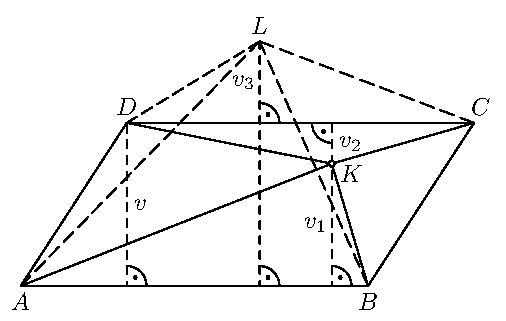
\includegraphics{obrazky/62K2}

Obr. 4
\end{center}
Trojuholníky $ABL$ a $DCL$ majú zhodné strany $AB$ a $CD$. Ak $v_3$ označuje príslušnú výšku druhého z~nich, je výška prvého z~nich rovná $v + v_3$, takže pre rozdiel obsahov týchto trojuholníkov platí
\begin{align*}
S_{ABL} - S_{DCL} &= \frac{1}{2} |AB| \cdot (v~+ v_3 ) - \frac{1}{2}|CD|\cdot v_3 =\frac{1}{2} |AB| \cdot (v~+ v_3 - v_3 ) =\\
&= \frac{1}{2} |AB| \cdot v~= \frac{1}{2} S_{ABCD} = S_{BCK} + S_{DAK}.
\end{align*}
Odtiaľ vyplýva
$$S_{ABL} = S_{BCK} + S_{DAK} + S_{DCL} = 60\,\text{cm}^2.$$
\\
\kom Úloha precvičuje použitie tvrdenia, ktoré sme dokázali v~prvom geometrickom seminári, a to, že ak majú dva trojuholníky základňu rovnakej dĺžky, potom ich obsahy sú v~rovnakom pomere ako ich výšky na túto základňu.\\
\\
\begin{tcolorbox}[breakable,notitle,boxrule=0pt,colback=light-gray,colframe=light-gray]\ul{11.3} [64-S-2] Označme $K$ a $L$ postupne body strán $BC$ a $AC$ trojuholníka $ABC$, pre ktoré platí $|BK|= \frac{1}{3}|BC|$, $|AL| =\frac{1}{3}|AC|$. Nech $M$ je priesečník úsečiek $AK$ a $BL$. Vypočítajte pomer obsahov trojuholníkov $ABM$ a $ABC$.

\end{tcolorbox}

\rieh Označme $v$ výšku trojuholníka $ABC$ na stranu $AB$, $v_1$ výšku trojuholníka $ABM$ na stranu $AB$ a $v_2$ výšku trojuholníka $KLM$ na stranu $KL$ (obr. 5). Z~podobnosti trojuholníkov $LKC$ a $ABC$ (zaručenej vetou $sus$) vyplýva, že $|KL| =\frac{2}{3} |AB|$. Z~porovnania ich výšok zo spoločného vrcholu $C$ vidíme, že výška $v$ trojuholníka $ABC$ je rovná trojnásobku vzdialenosti priečky $KL$ od strany $AB$, teda $v = 3(v_1 +v_2)$. Keďže $AK$ a $BL$ sú priečky rovnobežiek $KL$ a $AB$, vyplýva zo zhodnosti prislúchajúcich striedavých uhlov podobnosť trojuholníkov $ABM$ a $KLM$.
\begin{center}
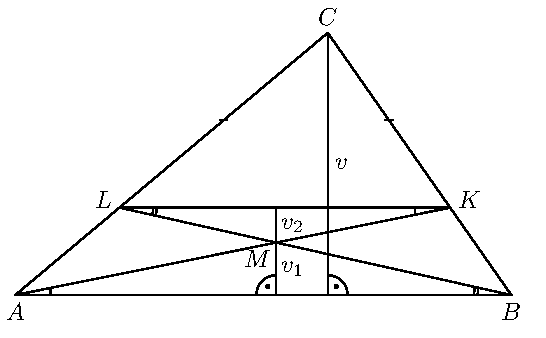
\includegraphics{obrazky/64S2}

Obr. 5
\end{center}
Keďže $|KL| =\frac{2}{3}|AB|$, je tiež $v_2 =\frac{2}{3}v_1$, a preto $v_1 + v_2 =\frac{5}{3}v_1$, čiže
$$v = 3(v_1 + v_2) = 5v_1.$$
Trojuholníky $ABM$ a $ABC$ majú spoločnú stranu $AB$, preto ich obsahy sú v~pomere výšok na túto stranu, takže obsah trojuholníka $ABC$ je päťkrát väčší ako obsah trojuholníka $ABM$.\\
\\
\kom Ďalšia úloha, ktorá precvičuje rovnaké tvrdenie ako predchádzajúca. Pomery výšok je tentoraz potrebné určiť z~podobnosti trojuholníkov. Tu sa teda uplatnia znalosti precvičované na minulom seminárnom stretnutí. \\
\\
\begin{tcolorbox}[breakable,notitle,boxrule=0pt,colback=light-gray,colframe=light-gray]\ul{11.4} [64-II-3]  Daný je lichobežník $ABCD$ so základňami $AB$, $CD$, pričom $2|AB| = 3|CD|$.

a) Nájdite bod $P$ vnútri lichobežníka tak, aby obsahy trojuholníkov $ABP$ a $CDP$ boli v~pomere $3 : 1$ a aj obsahy trojuholníkov $BCP$ a $DAP$ boli v~pomere $3 : 1$.

b) Pre nájdený bod $P$ určte postupný pomer obsahov trojuholníkov $ABP$, $BCP$, $CDP$ a $DAP$.

\end{tcolorbox}

\rieh Predpokladajme, že bod $P$ má požadované vlastnosti. Priamka rovnobežná so základňami lichobežníka a prechádzajúca bodom $P$ pretína ramená $AD$ a $BC$ postupne v~bodoch $M$ a $N$ (obr. 6). Označme $v$ výšku daného lichobežníka, $v_1$ výšku trojuholníka $CDP$ a $v_2$ výšku trojuholníka $ABP$.
\begin{center}
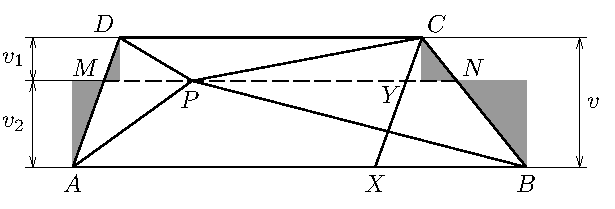
\includegraphics{obrazky/64K3}

Obr. 6
\end{center}
a) Keďže obsahy trojuholníkov $ABP$ a $CDP$ sú v~pomere $3 : 1$, platí
$$\frac{|AB|v_2}{2}:\frac{|CD|v_1}{2}= 3 : 1, \ \ \ \ \text{čiže} \ \ \ \ \frac{v_1}{v_2}=\frac{1}{3}\cdot \frac{|AB|}{|CD|}=\frac{1}{3}\cdot \frac{3}{2}=\frac{1}{2}.$$
Z~vyznačených dvojíc podobných pravouhlých trojuholníkov vyplýva, že v~práve určenom pomere $2 : 1$ výšok $v_2$ a $v_1$ delí aj bod $M$ rameno $AD$ a bod $N$ rameno $BC$ (v~prípade pravého uhla pri jednom z~vrcholov $A$ či $B$ je to zrejmé rovno). Tým je konštrukcia bodov $M$ a $N$, a teda aj úsečky $MN$ určená. Teraz zistíme, v~akom pomere ju delí uvažovaný bod $P$.

Keďže obsahy trojuholníkov $BCP$ a $DAP$ sú v~pomere $3 : 1$, platí
$$ \bigg(\frac{|NP|v_1}{2}+\frac{|NP|v_2}{2}\bigg): \bigg(\frac{|MP|v_1}{2}+\frac{|MP|v_2}{2}\bigg)= 3 : 1,$$
$$ \frac{|NP|(v_1 + v_2 )}{2}: \frac{|MP|(v_1 + v_2 )}{2}= 3 : 1, \ \ \ \  |NP| : |MP| = 3 : 1.$$
Tým je konštrukcia (jediného) vyhovujúceho bodu $P$ úplne opísaná.

b) Doplňme trojuholník $DAC$ na rovnobežník $DAXC$. Jeho strana $CX$ delí priečku $MN$ na dve časti, a keďže $v_1 =\frac{1}{3}v$, môžeme dĺžku priečky $MN$ vyjadriť ako $|MN| = |MY | + |Y N| = |AX| +\frac{1}{3} |XB| = |CD| +\frac{1}{3} (|AB| - |CD|) = \frac{1}{3}|AB| +\frac{2}{3}|CD| = \frac{7}{6}|CD|$, lebo podľa zadania platí $|AB| =\frac{3}{2}|CD|$. Preto
$$|MP| =\frac{1}{4}|MN| =\frac{1}{4} \cdot \frac{7}{6}|CD| = \frac{7}{24}|CD|,$$
takže pre pomer obsahov trojuholníkov $CDP$ a $DAP$ platí
$$ \frac{|CD|v_1}{2}:\frac{|MP|(v_1 + v_2 )}{2}= (|CD|v_1 ) : \bigg( \frac{7}{24}\cdot |CD| \cdot 3v_1\bigg)= 1 :\frac{7}{8} = 8 : 7.$$
Pomer obsahov trojuholníkov $BCP$ a $CDP$ je teda $21 : 8$ a pomer obsahov trojuholníkov $ABP$ a $BCP$ je tak $24 : 21$. Postupný pomer obsahov trojuholníkov $ABP$, $BCP$, $CDP$ a $DAP$ je preto $24 : 21 : 8 : 7$.\\
\\
\kom Táto komplexná úloha je vrcholom tohto seminárneho stretnutia. Vyžaduje umnú prácu s~pomermi obsahov, podobnými trojuholníkmi aj netriviálny nápad doplnenia trojuholníka $DAC$ na rovnobežník. Je tak vhodné skôr než samostatne úlohu riešiť spoločne na tabuľu. Študentom tiež pripomenieme, že podobne ako v~úvodnej úlohe, aj tu našlo vhodné rozdelenie zadaného útvaru svoje opodstatnenie a prispelo k~úspešnému rozklúsknutiu problému. \\
\\
\begin{tcolorbox}[breakable,notitle,boxrule=0pt,colback=light-gray,colframe=light-gray]\ul{11.5} [62-I-6] Vnútri pravidelného šesťuholníka $ABCDEF$ s~obsahom 30\,cm$^2$ je zvolený bod $M$. Obsahy trojuholníkov $ABM$ a $BCM$ sú postupne 3\,cm$^2$ a 2\,cm$^2$. Určte obsahy trojuholníkov $CDM$, $DEM$, $EFM$ a $FAM$.

\end{tcolorbox}

\rieh Úloha je o~obsahu šiestich trojuholníkov, na ktoré je daný pravidelný šesťuholník rozdelený spojnicami jeho vrcholov s~bodom $M$ (obr. 7). Celý šesťuholník s~daným obsahom, ktorý označíme $S$, možno rozdeliť na šesť rovnostranných trojuholníkov s~obsahom $S/6$ (obr. 8). Ak označíme $r$ ich stranu, $v$ vzdialenosť rovnobežiek $AB$, $CD$ a $v_1$ vzdialenosť bodu $M$ od priamky $AB$, dostaneme
$$S_{ABM} + S_{EDM} =\frac{1}{2}rv_1 +\frac{1}{2}r(v - v_1 ) = \frac{1}{2} rv =\frac{S}{3},$$
lebo $S/3$ je súčet obsahov dvoch vyfarbených rovnostranných trojuholníkov. Vďaka symetrii majú tú istú hodnotu $S/3$ aj súčty $S_{BCM} +S_{EFM}$ a $S_{CDM} +S_{FAM}$. Odtiaľ už dostávame prvé dva neznáme obsahy $S_DEM = S/3 - S_{ABM} = 7$\,cm$^2$ a $S_{EFM}= S/3 - S_{BCM} = 8$\,cm$^2$.
\begin{center}
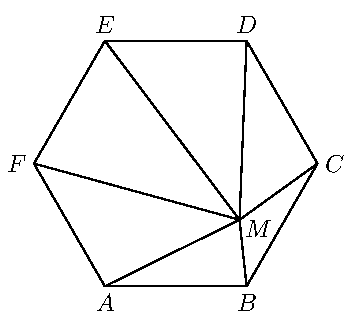
\includegraphics{obrazky/62D61} 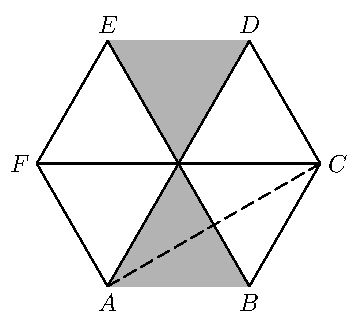
\includegraphics{obrazky/62D62}\\

Obr. 7  \hspace{160pt} Obr. 8
\end{center}
Ako určiť zvyšné dva obsahy $S_{CDM}$ a $S_{FAM}$, keď zatiaľ poznáme len ich súčet $S/3$? Všimnime si, že súčet zadaných obsahov trojuholníkov $ABM$ a $BCM$ má významnú hodnotu $S/6$, ktorá je aj obsahom trojuholníka $ABC$ (to vyplýva opäť z~obr. 8). Taká zhoda obsahov znamená práve to, že bod $M$ leží na uhlopriečke $AC$. Trojuholníky $ABM$ a $BCM$ tak majú zhodné výšky zo spoločného vrcholu $B$ a to isté platí aj pre výšky trojuholníkov $CDM$ a $FAM$ z~vrcholov $F$ a $D$ ( t.\,j. bodov, ktoré majú od priamky $AC$ rovnakú vzdialenosť). Pre pomery obsahov týchto dvojíc trojuholníkov tak dostávame
$$\frac{S_{CDM}}{S_{FAM}}=\frac{|CM|}{|AM|}=\frac{S_{BCM}}{S_{ABM}}=\frac{2}{3}.$$
V~súčte $S_{CDM} + S_{FAM}$ majúcom hodnotu $S/3$ sú teda sčítance v~pomere $2 : 3$. Preto $S_{CDM} =4$\,cm$^2$ a $S_{FAM} = 6$\,cm$^2$.\\
\\
\kom Úloha je odľahčeným a netradičným príkladom využitia princípu, na ktorom sme stavali celé toto seminárne stretnutie: súčty obsahov \uv{protiľahlých} trojuholníkov sú stále rovnaké. Posledná časť úlohy vyžaduje netriviálny nápad a študenti tak možno budú potrebovať malú radu.
\subsection*{Domáca práca}
\begin{tcolorbox}[breakable,notitle,boxrule=0pt,colback=light-gray,colframe=light-gray]\ul{11.6} [65-I-4] Vnútri strán $AB$, $AC$ daného trojuholníka $ABC$ sú zvolené postupne body $E$, $F$, pričom $EF \parallel BC$. Úsečka $EF$ je potom rozdelená bodom $D$ tak, že platí $$p = |ED| : |DF | = |BE| : |EA|.$$

a) Ukážte, že pomer obsahov trojuholníkov $ABC$ a $ABD$ je pre $p = 2 : 3$ rovnaký ako pre $p = 3 : 2$.

b) Zdôvodnite, prečo pomer obsahov trojuholníkov $ABC$ a $ABD$ má hodnotu aspoň 4.

\end{tcolorbox}

\rieh Pre spoločnú hodnotu $p$ oboch pomerov zo zadania platí
$$|ED| = p|DF| \ \ \ \ \text{a zároveň} \ \ \ \ |BE| = p|EA|.  \ \ \ \ (1)$$
Pred vlastným riešením oboch úloh a) a b) vyjadríme pomocou daného čísla $p$ skúmaný pomer obsahov trojuholníkov $ABC$ a $ABD$. Ten je rovný -- keďže trojuholníky majú spoločnú stranu AB -- pomeru dĺžok ich výšok $CC_0$ a $DD_0$ (obr. XXX), ktorý je rovnaký ako
\\
OBRAZOK
\\
pomer dĺžok úsečiek $BC$ a $ED$, a to na základe podobnosti pravouhlých trojuholníkov $BCC_0$ a $EDD_0$ podľa vety $uu$ (uplatnenej vďaka $BC \parallel ED$).\footnote{V prípade pravých uhlov $ABC$ a $AED$ to platí triviálne, lebo vtedy $B = C_0$ a $E = D0$.} Platí teda rovnosť
$$\frac{S_{ABC}}{S_{ABD}} =\frac{|BC|}{|ED|}.\ \ \ \  (2)$$
Vráťme sa teraz k~rovnostiam (1), podľa ktorých
$$|EF| = (1 + p)|DF| \ \ \ \ \text{a} \ \ \ \ |AB| = (1 + p)|EA|,$$
a všimnime si, že trojuholníky $ABC$ a $AEF$ majú spoločný uhol pri vrchole $A$ a zhodné uhly pri vrcholoch $C$ a $F$ (pretože $BC \parallel EF$), takže sú podľa vety $uu$ podobné. Preto
pre dĺžky ich strán platí
$$\frac{|AB|}{|AE|}=\frac{|BC|}{|EF|},\ \ \ \ \text{čiže} \ \ \ \  1 + p =\frac{|BC|}{(1 + p)|DF|}, \ \ \ \ \text{odkiaľ} \ \ \ \ |BC| = (1 + p)^2 |DF|.$$
Keď vydelíme posledný vzťah hodnotou $|ED|$, ktorá je rovná $p|DF|$ podľa (1), získame podiel z~pravej strany (2) a tým aj hľadané vyjadrenie
$$\frac{S_{ABC}}{S_{ABD}}=\frac{(1 + p)^2}{p}. \ \ \ \  (3)$$

a) Algebraickou úpravou zlomku zo vzťahu (3)
$$ \frac{(1 + p)^2}{p}=\frac{1 + 2p + p^2}{p}= 2 + p + \frac{1}{p}$$
zisťujeme, že hodnota pomeru $S_{ABC} : S_{ABD}$ je pre akékoľvek dve navzájom prevrátené hodnoty $p$ a $1/p$ rovnaká, teda nielen pre hodnoty $2/3$ a $3/2$, ako sme mali ukázať.

b) Podľa vzťahu (3) je našou úlohou overiť pre každé $p > 0$ nerovnosť
$$\frac{(1 + p)^2}{p}\geq4,\ \ \ \ \text{čiže} \ \ \ \  (1 + p)^2\geq 4p.$$
To je však zrejme ekvivalentné s~nerovnosťou $(1 -p)^2\geq 0$, ktorá skutočne platí, nech je základ druhej mocniny akýkoľvek (rovnosť nastane jedine pre $p = 1$).

Dodajme, že pre iný dôkaz bolo možné využiť aj vyššie uvedené \uv{symetrické} vyjadrenie
$$\frac{(1 + p)^2}{p}= 2 + p +\frac{1}{p}$$
a uplatniť naň dobre známu nerovnosť $p + 1/p \geq 2$, ktorej platnosť pre každé $p > 0$ vyplýva napr. z~porovnania aritmetického a geometrického priemeru dvojice čísel $p$ a $1/p$, nazývaného AG-nerovnosť:
$$\frac{1}{2}\bigg(p +\frac{1}{p}\bigg)\geq \sqrt{p\cdot \frac{1}{p}}= 1, \ \ \ \ \text{pretože všeobecne} \ \ \ \ \frac{a+b}{2} \geq \sqrt{a\cdot b} \ \ \ \ (\forall a, b \geq 0).$$

\subsection*{Doplňujúce zdroje a materiály}
Rovnako ako v~predchádzajúcich geometrických seminároch ostávame v~odporúčaniach verní publikáciám [~\cite{andreescu2013}] a [~\cite{kadlecek1996}].

